\chapter{真核细胞的功能组织}\label{ch:b1:eukaryotic-cell}

胰腺中的一个\omterm{def:b1:cell-unit-of-life:cell}{细胞}每天制造
约与自身质量相当的消化酶，
并将其分泌到\omterm{def:b1:flowering-plant-organization:tissues}{导管}中。这些酶本身是蛋白质，足以消化制造它们的\omterm{def:b1:cell-unit-of-life:cell}{细胞}；
因此\omterm{def:b1:cell-unit-of-life:cell}{细胞}将其合成于一层封闭的膜之内，
再经由第二个区室运送，在那里分拣、浓缩，
以颗粒形式储存，只在进餐信号到来时才释放。
每一步都在不同的膜包围空间中进行，
空间之间的物质转运由囊泡承担。本章介绍\omterm{def:b1:cell-unit-of-life:prokeuk}{真核细胞}的各个区室、
蛋白质流经的\omterm{def:b1:eukaryotic-cell:endomembrane}{内膜系统}、转化能量的\omterm{def:b1:eukaryotic-cell:organelle}{细胞器}、
维持\omterm{def:b1:cell-unit-of-life:cell}{细胞}形态并驱动其各部分运动的骨架，
以及区分植物\omterm{def:b1:cell-unit-of-life:cell}{细胞}与动物\omterm{def:b1:cell-unit-of-life:cell}{细胞}的
特征。

\section{区室}

\begin{definition}[细胞器，细胞溶胶]\label{def:b1:eukaryotic-cell:organelle}
\emph{细胞器}\index{细胞器}是\omterm{def:b1:cell-unit-of-life:cell}{细胞}内具有确定组成和功能的结构，有膜包围的
\omterm{def:b1:cell-unit-of-life:cell}{细胞}器是一些区室，其内部成分
不同于
\emph{细胞溶胶}\index{细胞溶胶}，即位于其外部的\omterm{def:b1:cell-unit-of-life:cell}{细胞质}水溶液。有膜区室包括：
\omterm{def:b1:eukaryotic-cell:nucleus}{细胞核}、
\omterm{def:b1:eukaryotic-cell:endomembrane}{内质网}、\omterm{def:b1:eukaryotic-cell:endomembrane}{高尔基体}、\omterm{def:b1:eukaryotic-cell:endomembrane}{溶酶体}、\omterm{def:b1:eukaryotic-cell:peroxisome}{过氧化物酶体}、
\omterm{def:b1:eukaryotic-cell:mitochondrion}{线粒体}，植物中另有\omterm{def:b1:eukaryotic-cell:plastid}{质体}和\omterm{def:b1:eukaryotic-cell:plantcell}{液泡}。无膜\omterm{def:b1:cell-unit-of-life:cell}{细胞}器
包括核糖体、\omterm{def:b1:eukaryotic-cell:cytoskeleton}{中心体}和\omterm{def:b1:eukaryotic-cell:cytoskeleton}{细胞骨架}。
\end{definition}

\begin{omfigure}
\begin{tikzpicture}
  \node[anchor=south west, inner sep=0] (img) at (0,0)
    {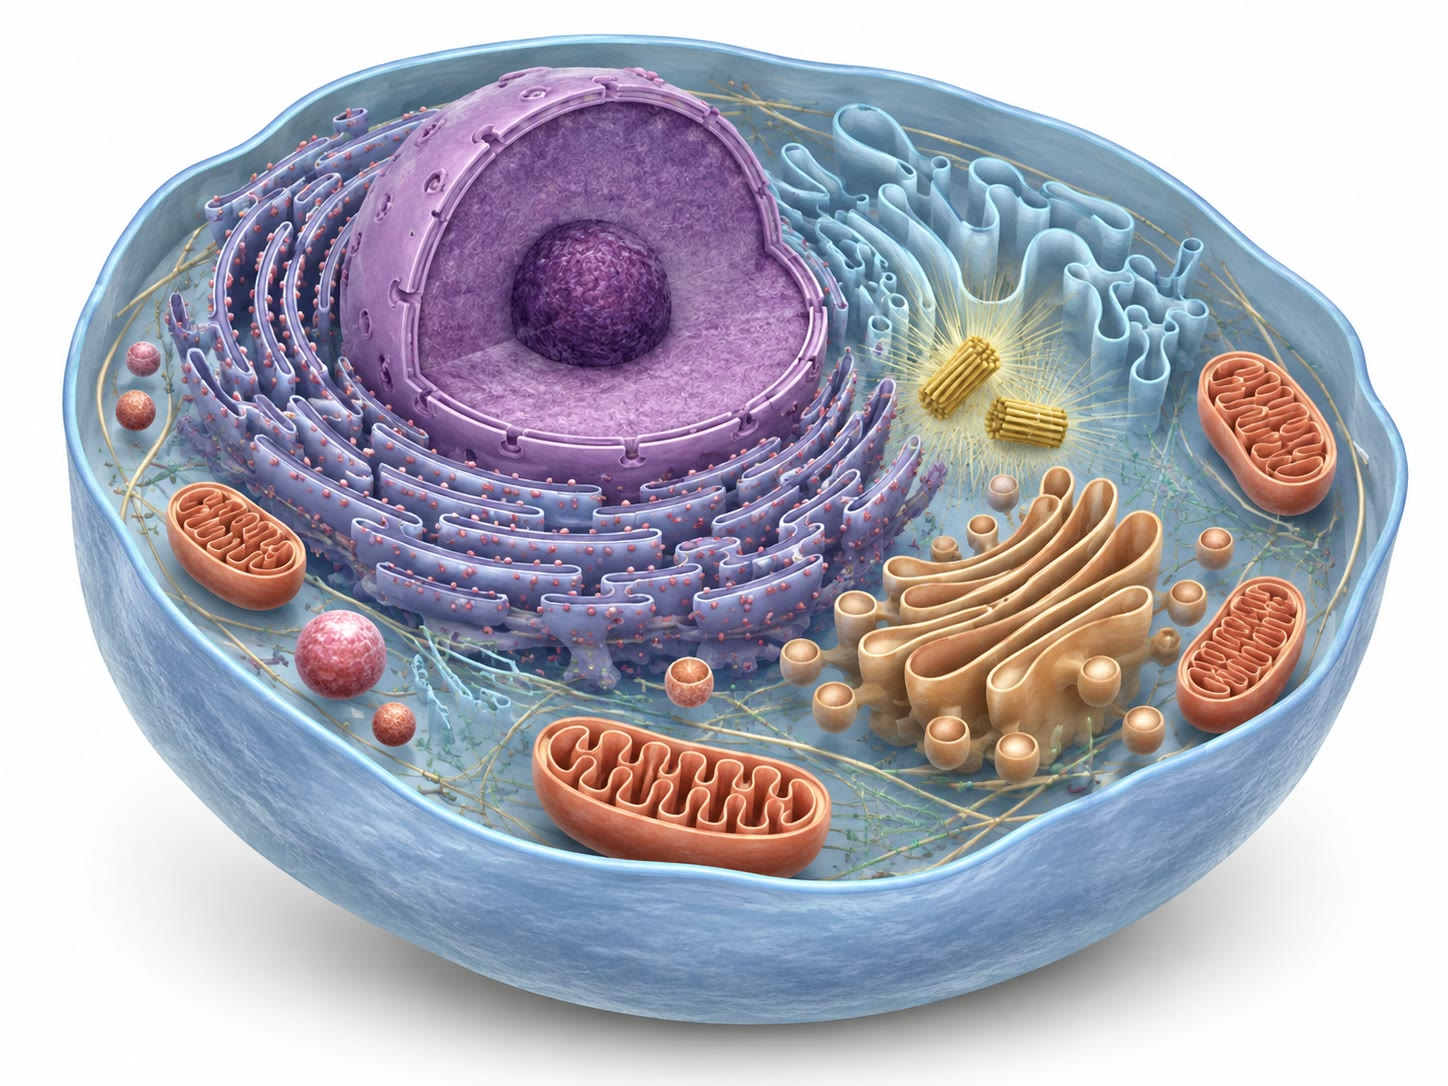
\includegraphics[width=0.6\linewidth]{images/book3/ai/fig-animal-cell-cutaway.jpg}};
  \begin{scope}[x={(img.south east)}, y={(img.north west)},
      every node/.style={font=\small}]
    \draw[omDef, thick] (0.42,0.72) -- (0.42,1.08) node[above] {细胞核、核仁、核孔};
    \draw[omDef, thick] (0.30,0.52) -- (-0.03,0.44) node[left, align=right] {粗面内质网};
    \draw[omDef, thick] (0.23,0.42) -- (-0.03,0.22) node[left] {溶酶体};
    \draw[omDef, thick] (0.07,0.62) -- (-0.03,0.76) node[left] {质膜};
    \draw[omDef, thick] (0.75,0.80) -- (1.03,0.88) node[right] {滑面内质网};
    \draw[omDef, thick] (0.69,0.63) -- (1.03,0.62) node[right] {中心体};
    \draw[omDef, thick] (0.87,0.42) -- (1.03,0.36) node[right] {线粒体};
    \draw[omDef, thick] (0.70,0.40) -- (0.80,-0.08) node[below] {高尔基体和囊泡};
    \draw[omDef, thick] (0.47,0.25) -- (0.35,-0.08) node[below] {线粒体};
  \end{scope}
\end{tikzpicture}

{\small 动物\omterm{def:b1:cell-unit-of-life:cell}{细胞}剖面示意图。\omterm{def:b1:eukaryotic-cell:nucleus}{细胞核}位于中央；
其周围是与\omterm{def:b1:eukaryotic-cell:nucleus}{核膜}相连的\omterm{def:b1:eukaryotic-cell:endomembrane}{粗面内质网}、
\omterm{def:b1:eukaryotic-cell:endomembrane}{滑面内质网}、\omterm{def:b1:eukaryotic-cell:endomembrane}{高尔基体}堆叠及其囊泡、
\omterm{def:b1:eukaryotic-cell:mitochondrion}{线粒体}、\omterm{def:b1:eukaryotic-cell:endomembrane}{溶酶体}，以及\omterm{def:b1:eukaryotic-cell:cytoskeleton}{中心体}，
\omterm{def:b1:eukaryotic-cell:cytoskeleton}{微管}自其向外辐射。}
\end{omfigure}

\begin{definition}[细胞核]\label{def:b1:eukaryotic-cell:nucleus}
\emph{细胞核}\index{细胞核}以\emph{染色质}\index{染色质}的形式容纳染色体，
即缠绕在组蛋白上的 DNA
（见\cref{ch:b1:genomes}）。\omterm{def:b1:cell-unit-of-life:cell}{细胞}核由\emph{核
膜}\index{核膜}包围，它由两层膜构成，外层膜与\omterm{def:b1:eukaryotic-cell:endomembrane}{内质网}相连，
膜上穿有\emph{核
孔}\index{核孔}，RNA 与蛋白质在调控下双向通过。
\emph{核仁}\index{核仁}是
合成核糖体 RNA 并装配核糖体的区域。\omterm{def:b1:cell-unit-of-life:cell}{细胞}核
将转录（在核内）与翻译（在核外）分隔开，
原核生物则没有这种分隔。
\end{definition}

\begin{proposition}[肝细胞的各个区室]\label{prop:b1:eukaryotic-cell:budget}
在一个体积为 \qty{5000}{\micro m^3} 的肝\omterm{def:b1:cell-unit-of-life:cell}{细胞}中，\omterm{def:b1:eukaryotic-cell:organelle}{细胞溶胶}约占
一半体积，\omterm{def:b1:eukaryotic-cell:mitochondrion}{线粒体}占五分之一，\omterm{def:b1:eukaryotic-cell:endomembrane}{内质网}占
六分之一，\omterm{def:b1:eukaryotic-cell:nucleus}{细胞核}占十六分之一，\omterm{def:b1:eukaryotic-cell:endomembrane}{高尔基体}、\omterm{def:b1:eukaryotic-cell:endomembrane}{溶酶体}和\omterm{def:b1:eukaryotic-cell:peroxisome}{过氧化物酶体}
合计约占百分之几。膜的分布则另有情况：在\omterm{def:b1:cell-unit-of-life:cell}{细胞}的
\qty{110000}{\micro m^2} 膜中，一半属于\omterm{def:b1:eukaryotic-cell:endomembrane}{内质网}，
约三分之一为\omterm{def:b1:eukaryotic-cell:mitochondrion}{线粒体}内膜，而\omterm{def:b1:cell-unit-of-life:cell}{质膜}仅占
\qty{2}{\%}。\omterm{def:b1:cell-unit-of-life:cell}{细胞}的大部分膜位于
\omterm{def:b1:cell-unit-of-life:cell}{细胞}内部。
\end{proposition}

\begin{omfigure}
\begin{tikzpicture}
\begin{axis}[
  xbar, bar width=8pt,
  width=0.72\linewidth, height=6.4cm,
  axis x line=bottom, axis y line=left,
  xmin=0, xmax=45, xlabel={细胞全部膜的占比（\%）},
  xlabel style={font=\small, at={(axis description cs:0.5,-0.13)}, anchor=north},
  symbolic y coords={nuclear envelope, plasma membrane, lysosomes and peroxisomes, Golgi apparatus, mitochondrial outer membrane, smooth ER, mitochondrial inner membrane, rough ER},
  ytick=data, yticklabels={核膜, 质膜, 溶酶体和过氧化物酶体, 高尔基体, 线粒体外膜, 光面内质网, 线粒体内膜, 粗面内质网}, tick label style={font=\small},
  enlarge y limits=0.08, xtick={0,10,20,30,40},
  nodes near coords, nodes near coords style={font=\scriptsize, anchor=west},
]
\addplot[fill=omDef!45, draw=omDef] coordinates
  {(0.2,nuclear envelope) (2,plasma membrane) (1.5,lysosomes and peroxisomes) (7,Golgi apparatus) (7,mitochondrial outer membrane) (16,smooth ER) (32,mitochondrial inner membrane) (35,rough ER)};
\end{axis}
\end{tikzpicture}

{\small 肝\omterm{def:b1:cell-unit-of-life:cell}{细胞}的膜分布情况。\omterm{def:b1:cell-unit-of-life:cell}{质膜}是唯一可从外部看到的膜，
占全部膜的百分之二；\omterm{def:b1:eukaryotic-cell:endomembrane}{内质网}和向内折叠的\omterm{def:b1:eukaryotic-cell:mitochondrion}{线粒体}内膜
合计占五分之四。}
\end{omfigure}

\section{内膜系统}

\begin{definition}[内质网、高尔基体、溶酶体]\label{def:b1:eukaryotic-cell:endomembrane}
\emph{内质网}\index{内质网}（ER）是
由膜片和膜管构成的网络，包围着一个连续的空间，
即管腔，并与\omterm{def:b1:eukaryotic-cell:nucleus}{核膜}相连。其
\emph{粗面}\index{粗面内质网}部分附有
核糖体，将其合成的蛋白质注入管腔或
膜中；其\emph{滑面}\index{滑面内质网}部分
合成脂质、储存钙并负责解毒。\emph{高尔
基体}\index{高尔基体}是由扁平膜囊堆叠而成的结构，
一端为靠近内质网的接收面（\emph{顺面}），另一端为
输出面（\emph{反面}），来自内质网的蛋白质在其中被修饰（糖链被修剪并添加），
再经分拣，装入囊泡，
运往各自的目的地。\emph{溶酶体}\index{溶酶体}是酸性囊泡（pH
$\approx 5$），内含大量水解酶，用以消化从外部摄入的物质
或衰老的\omterm{def:b1:eukaryotic-cell:organelle}{细胞器}。这些囊泡在区室之间、以及区室与\omterm{def:b1:cell-unit-of-life:cell}{质膜}之间往来，
共同构成
\emph{内膜系统}\index{内膜系统}：一组相连的区室，
其管腔在拓扑意义上相当于\omterm{def:b1:cell-unit-of-life:cell}{细胞}外部。
\end{definition}

\begin{proposition}[分泌途径]\label{prop:b1:eukaryotic-cell:secretory}
\index{分泌途径}
需要分泌、运往\omterm{def:b1:cell-unit-of-life:cell}{质膜}或运往\omterm{def:b1:eukaryotic-cell:endomembrane}{溶酶体}的蛋白质，
由附着在\omterm{def:b1:eukaryotic-cell:endomembrane}{粗面内质网}上的核糖体合成，合成时即进入\omterm{def:b1:eukaryotic-cell:endomembrane}{内质网}腔，
并在其中折叠，经囊泡运至\omterm{def:b1:eukaryotic-cell:endomembrane}{高尔基体}的顺面，
穿过堆叠的膜囊时被修饰，
最后从反面以囊泡形式离开，送往其目的地：
可能是在信号作用下与\omterm{def:b1:cell-unit-of-life:cell}{质膜}融合的分泌颗粒，
（\emph{调节性胞吐}\index{胞吐}），
可能是持续与\omterm{def:b1:cell-unit-of-life:cell}{质膜}融合的囊泡（\emph{组成性}胞吐，同时补充新的膜），
也可能是\omterm{def:b1:eukaryotic-cell:endomembrane}{溶酶体}。胞质蛋白和核蛋白在游离核糖体上合成，
从不进入这一系统。决定去向的是
蛋白质起始端的\emph{信号序列}\index{信号序列}
（见\cref{ch:b1:gene-expression}）。
\end{proposition}
\begin{proof}[实验证据]
帕拉德（20 世纪 60 年代）用放射性氨基酸饲喂豚鼠胰腺切片，
历时三分钟（\emph{脉冲}），随后改用未标记的氨基酸（\emph{追踪}），
并在不同时间间隔取样，对电镜照片进行放射自显影以定位放射性。
在 \qty{3}{min} 时，银颗粒位于\omterm{def:b1:eukaryotic-cell:endomembrane}{粗面内质网}上；
在 \qty{20}{min} 时位于\omterm{def:b1:eukaryotic-cell:endomembrane}{高尔基体}上；
在 \qty{40}{min} 时位于浓缩\omterm{def:b1:eukaryotic-cell:plantcell}{液泡}和新生颗粒上；
在 \qty{2}{h} 时位于\omterm{def:b1:flowering-plant-organization:tissues}{导管}腔中。\omterm{def:b1:cell-unit-of-life:fractionation}{细胞分级分离}在化学上给出了相同的顺序。
布洛贝尔（20 世纪 70 年代）发现，在无膜的试管中合成的分泌蛋白，
比分泌形式长二十个残基，且不受外加蛋白酶的保护，
而在有\omterm{def:b1:eukaryotic-cell:endomembrane}{内质网}膜存在时合成的，
则被切除并受到保护：多出的残基是
引导生长中的肽链进入\omterm{def:b1:eukaryotic-cell:endomembrane}{内质网}的信号。
\end{proof}

\begin{omfigure}
\begin{tikzpicture}
\begin{axis}[
  width=0.9\linewidth, height=6.2cm,
  axis x line=bottom, axis y line=left,
  xmin=0, xmax=130, ymin=0, ymax=105,
  xlabel={脉冲后时间 (min)}, ylabel={标记所占比例 (\%)},
  xlabel style={font=\small, at={(axis description cs:0.5,-0.12)}, anchor=north},
  ylabel style={font=\small},
  tick label style={font=\small}, xtick={0,20,40,60,80,100,120}, ytick={0,25,50,75,100},
  legend style={font=\small, at={(0.5,-0.24)}, anchor=north, draw=none, legend columns=2, /tikz/every even column/.append style={column sep=0.4cm}},
  clip=false,
]
\addplot[very thick, omDef, smooth] coordinates {(3,88) (7,55) (15,25) (30,8) (60,2) (120,0)};
\addlegendentry{粗面内质网}
\addplot[very thick, omProp, smooth] coordinates {(3,8) (7,35) (15,55) (30,35) (60,10) (120,2)};
\addlegendentry{高尔基体与浓缩液泡}
\addplot[very thick, omThm, smooth] coordinates {(3,0) (7,3) (15,12) (30,45) (60,70) (90,55) (120,30)};
\addlegendentry{分泌颗粒}
\addplot[very thick, omExo, smooth] coordinates {(3,0) (7,0) (15,0) (30,2) (60,12) (90,35) (120,65)};
\addlegendentry{分泌入导管}
\end{axis}
\end{tikzpicture}

{\small 胰腺中的帕拉德脉冲-追踪实验：标记蛋白随时间的分布。
它们在四分之一小时内从\omterm{def:b1:eukaryotic-cell:endomembrane}{内质网}转运至\omterm{def:b1:eukaryotic-cell:endomembrane}{高尔基体}，
在一小时内到达颗粒，
并在随后两小时内离开\omterm{def:b1:cell-unit-of-life:cell}{细胞}。}
\end{omfigure}

\begin{omfigure}
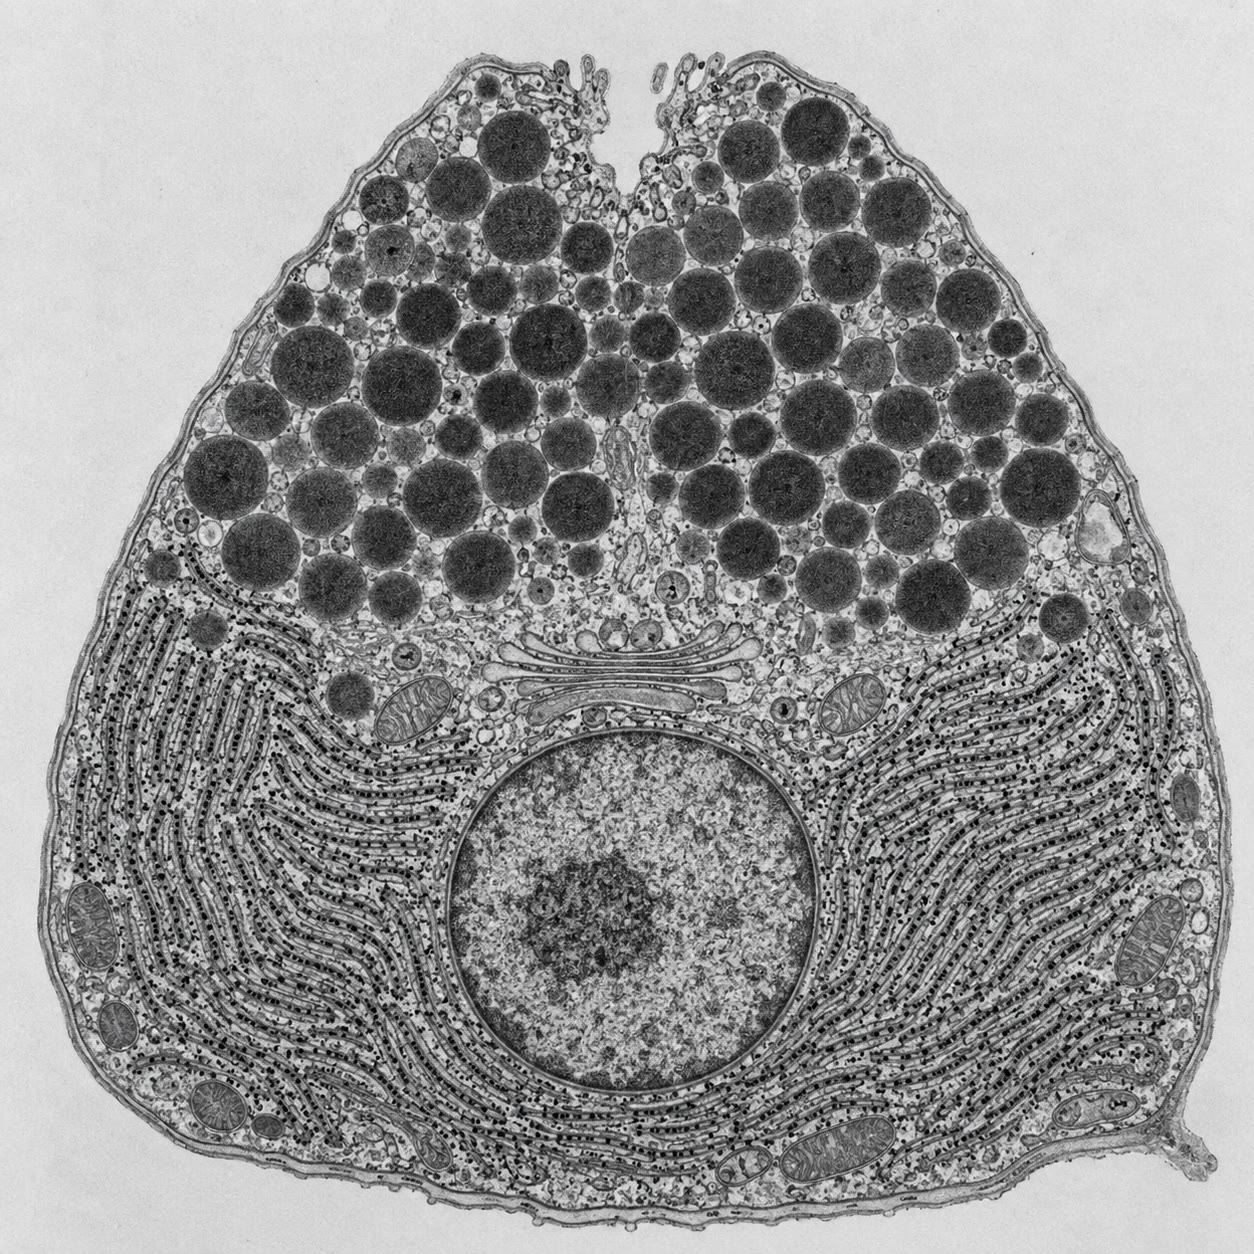
\includegraphics[width=0.44\linewidth]{images/book3/ai/b3-06-acinar-cell-tem.jpg}

{\small 胰腺腺泡\omterm{def:b1:cell-unit-of-life:cell}{细胞}的透射电镜图像：基部\omterm{def:b1:eukaryotic-cell:nucleus}{细胞核}周围平行排列的\omterm{def:b1:eukaryotic-cell:endomembrane}{粗面内质网}堆，
上方为\omterm{def:b1:eukaryotic-cell:endomembrane}{高尔基体}，
致密的分泌颗粒聚集于顶端，
并朝向\omterm{def:b1:flowering-plant-organization:tissues}{导管}一侧。}
\end{omfigure}

\begin{method}[追踪分子在细胞中的路径]\label{met:b1:eukaryotic-cell:pulsechase}
\begin{enumerate}
  \item 标记一批短期内产生的分子：将\omterm{def:b1:cell-unit-of-life:cell}{细胞}暴露于放射性或
        荧光前体数分钟（脉冲），随后
        换成过量未标记前体（追踪），使得
        只有脉冲期间合成的分子带有标记。
  \item 定时取样、固定，并定位标记：通过
        切片放射自显影、荧光显微术，或
        分级分离后计数。
  \item 标记峰最先出现的区室位于上游；
        峰的先后顺序即为路径，峰间的间隔即为
        转运时间。
  \item 阻断某一步骤（低温、能量抑制剂、突变体），观察
        标记在何处积累：积累处即为阻断点之前的区室。
\end{enumerate}
\end{method}

\begin{definition}[胞吞作用]\label{def:b1:eukaryotic-cell:endocytosis}
\emph{胞吞作用}\index{胞吞作用}将物质带入\omterm{def:b1:cell-unit-of-life:cell}{细胞}：\omterm{def:b1:cell-unit-of-life:cell}{质膜}
包裹该物质并内陷，脱离形成囊泡，
囊泡通常与\omterm{def:b1:eukaryotic-cell:endomembrane}{溶酶体}融合。\emph{吞噬作用}摄入颗粒
（如细菌、死亡\omterm{def:b1:cell-unit-of-life:cell}{细胞}）；\emph{胞饮作用}摄入
液滴；\emph{受体介导的胞吞作用}先使特定分子
（携带胆固醇的颗粒、携带铁的转铁蛋白）在有被小窝中的受体上富集，
然后将其摄入。胞吐作用向\omterm{def:b1:cell-unit-of-life:cell}{细胞}表面添加膜，
胞吞作用则移除膜；在分泌\omterm{def:b1:cell-unit-of-life:cell}{细胞}中，两者
保持平衡，使\omterm{def:b1:cell-unit-of-life:cell}{细胞}表面积保持恒定，而整片膜区域
每小时都在其中循环。
\end{definition}

\section{线粒体与质体}

\begin{definition}[线粒体]\label{def:b1:eukaryotic-cell:mitochondrion}
\emph{线粒体}\index{线粒体}是一种\omterm{def:b1:eukaryotic-cell:organelle}{细胞器}，
直径为 \qtyrange{0.5}{1}{\micro m}，长数微米，
由两层膜包被：光滑的外膜允许小分子通过，
内膜向内折叠形成\emph{嵴}\index{嵴}，
对离子不可渗透，并承载呼吸链和 ATP
合酶（见\cref{ch:b1:respiration-fermentation}）。其内部为
\emph{基质}\index{基质}，内含克雷布斯循环的酶、
细菌型核糖体以及若干拷贝的
小型环状 DNA。线粒体通过分裂增殖，沿
\omterm{def:b1:eukaryotic-cell:cytoskeleton}{细胞骨架}移动，每个\omterm{def:b1:cell-unit-of-life:cell}{细胞}的数量从几百到几千个不等。
\end{definition}

\begin{definition}[质体]\label{def:b1:eukaryotic-cell:plastid}
\emph{质体}\index{质体}是植物\omterm{def:b1:cell-unit-of-life:cell}{细胞}中具有双层膜的\omterm{def:b1:eukaryotic-cell:organelle}{细胞器}，
其中\emph{叶绿体}\index{叶绿体}内还有第三套膜系统，
即\emph{类囊体}\index{类囊体}，类囊体堆叠成基粒，
浸没于\emph{基质}\index{基质}中，负责
进行光合作用（\cref{ch:b1:photosynthesis}）；淀粉体储存
淀粉；有色体含有果实和花瓣的色素。所有
质体都由前质体发育而来，与\omterm{def:b1:eukaryotic-cell:mitochondrion}{线粒体}一样，具有自身的
环状 DNA 和细菌型核糖体，并通过分裂增殖。
\end{definition}

\begin{omfigure}
\begin{minipage}[b]{0.48\linewidth}\centering
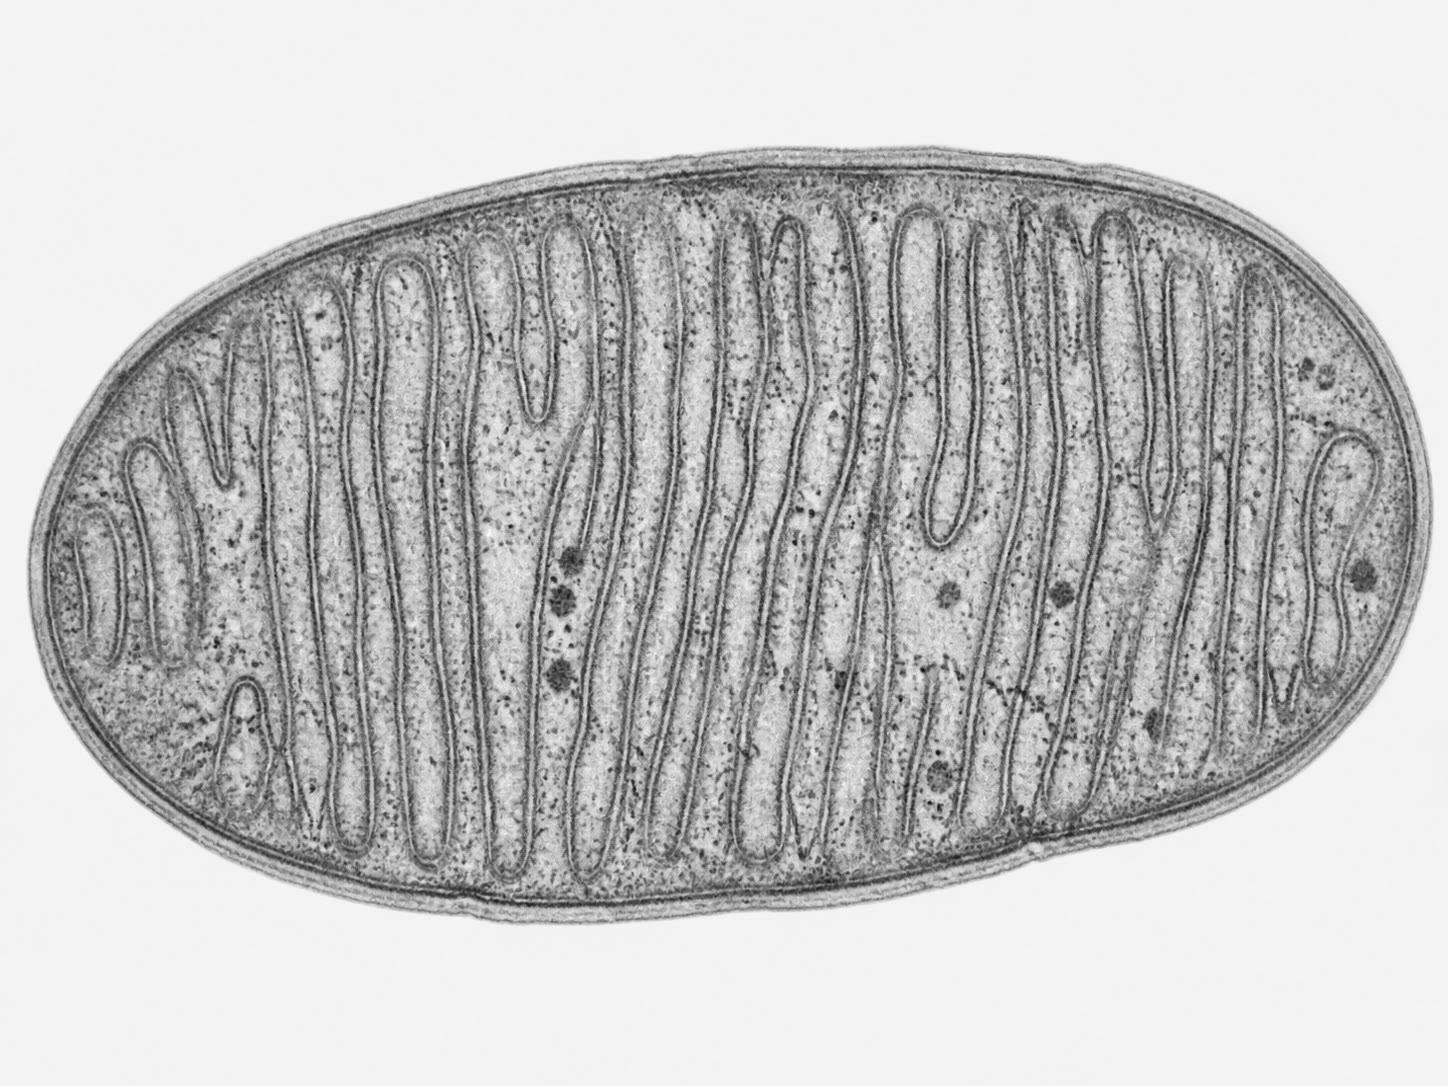
\includegraphics[width=0.96\linewidth]{images/book2/ai/g12-resp-mitochondrion-tem.jpg}
\end{minipage}\hfill
\begin{minipage}[b]{0.48\linewidth}\centering
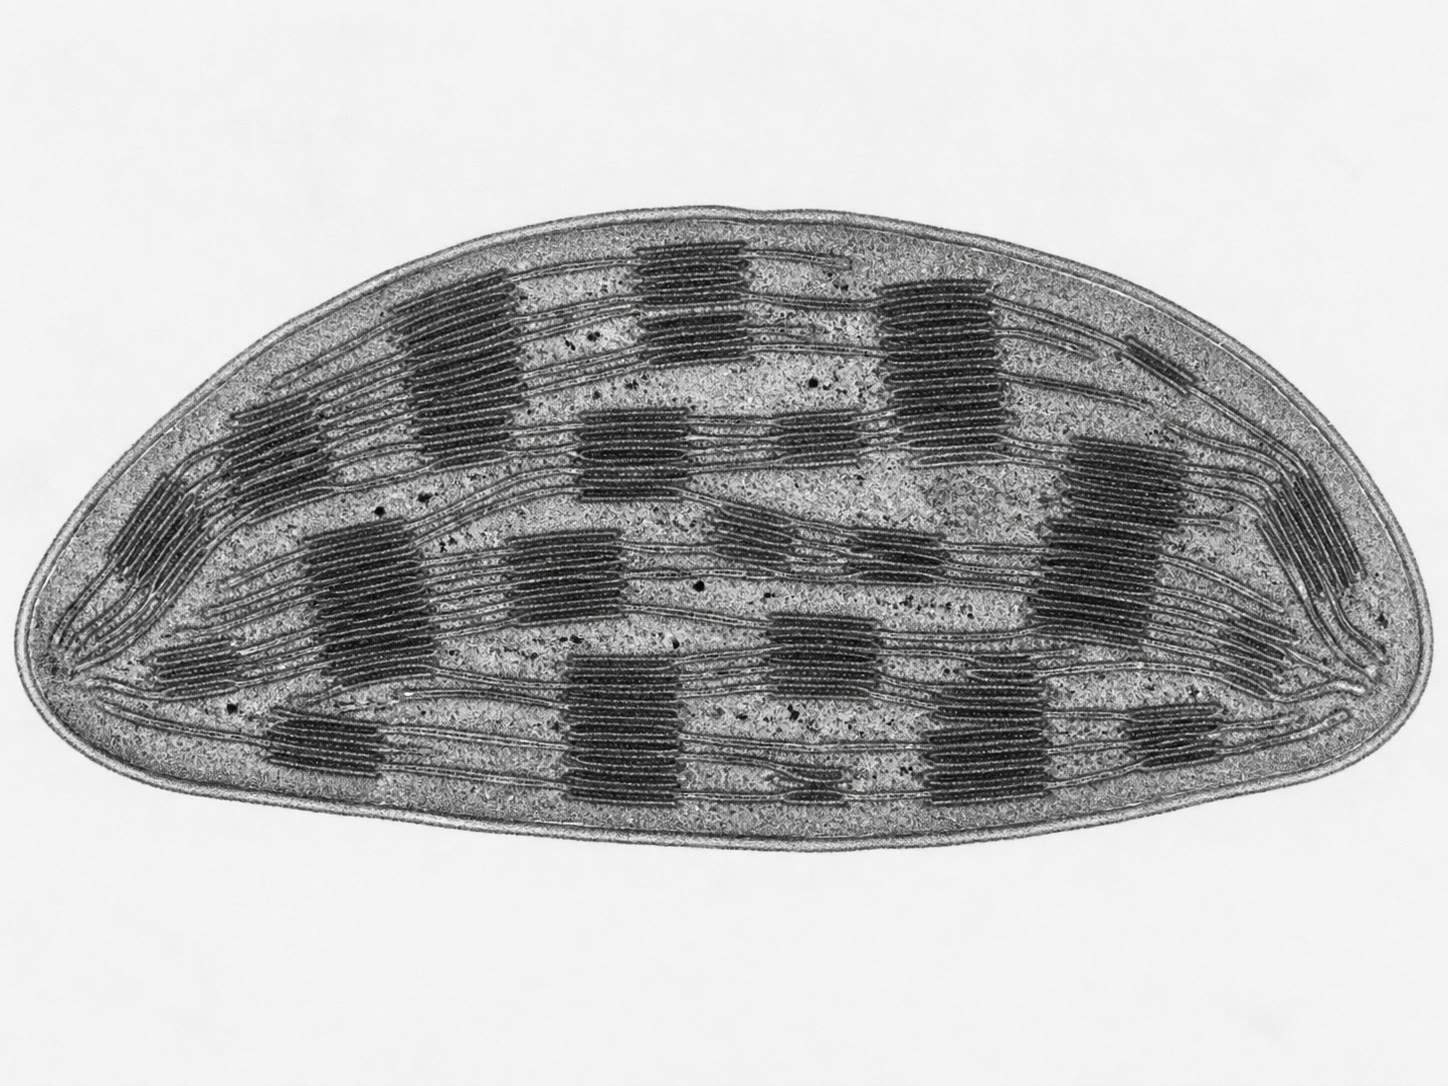
\includegraphics[width=0.96\linewidth]{images/book2/ai/g12-photo-chloroplast-tem.jpg}
\end{minipage}

{\small \omterm{def:b1:eukaryotic-cell:mitochondrion}{线粒体}（左）与\omterm{def:b1:eukaryotic-cell:plastid}{叶绿体}（右）的切面，
电镜下观察。两者均有两层包膜；内部分别为
\omterm{def:b1:eukaryotic-cell:mitochondrion}{线粒体}折叠的内膜与\omterm{def:b1:eukaryotic-cell:plastid}{叶绿体}堆叠的
\omterm{def:b1:eukaryotic-cell:plastid}{类囊体}——这些膜负责能量的
转换。}
\end{omfigure}

\begin{proposition}[内共生起源]\label{prop:b1:eukaryotic-cell:endosymbiosis}
\index{内共生}
\omterm{def:b1:eukaryotic-cell:mitochondrion}{线粒体}和\omterm{def:b1:eukaryotic-cell:plastid}{质体}源自自由生活的细菌，它们被祖先\omterm{def:b1:cell-unit-of-life:prokeuk}{真核细胞}
吞入并保留为共生体：\omterm{def:b1:eukaryotic-cell:mitochondrion}{线粒体}来自需氧细菌，
\omterm{def:b1:eukaryotic-cell:plastid}{质体}来自蓝细菌。
\end{proposition}
\begin{proof}[证据]
两种\omterm{def:b1:eukaryotic-cell:organelle}{细胞器}都具有两层膜：内膜具有细菌的组成，
外膜则类似宿主的膜；具有不含组蛋白的环状染色体；
核糖体的大小与对抗生素的敏感性与细菌一致；
遗传密码带有细菌的变体；以二分裂方式分裂，
独立于宿主\omterm{def:b1:cell-unit-of-life:cell}{细胞}的分裂；且其基因测序后，
测序后，其基因与特定细菌谱系的基因归为一组，
（α-变形菌纲、蓝细菌）聚在一起，而不是与
所居宿主\omterm{def:b1:cell-unit-of-life:cell}{细胞}的核基因聚在一起。它们的大部分原始基因
此后已转入\omterm{def:b1:eukaryotic-cell:nucleus}{细胞核}，\omterm{def:b1:eukaryotic-cell:organelle}{细胞器}已
无法独立生存。
\end{proof}

\begin{definition}[过氧化物酶体]\label{def:b1:eukaryotic-cell:peroxisome}
\emph{过氧化物酶体}\index{过氧化物酶体}是一种小型单层膜
\omterm{def:b1:eukaryotic-cell:organelle}{细胞器}，内含氧化酶，可将氢从
底物（脂肪酸、醇）转移给氧气，生成过氧化氢，
并含过氧化氢酶，就地分解过氧化氢。它
将危险的化学反应限制在\omterm{def:b1:eukaryotic-cell:organelle}{细胞器}之内。
\end{definition}

\section{细胞骨架}

\begin{definition}[细胞骨架]\label{def:b1:eukaryotic-cell:cytoskeleton}
\emph{细胞骨架}\index{细胞骨架}是由蛋白质纤维构成的网络，
它赋予\omterm{def:b1:cell-unit-of-life:cell}{细胞}形状，锚定其\omterm{def:b1:eukaryotic-cell:organelle}{细胞器}，并
移动\omterm{def:b1:eukaryotic-cell:organelle}{细胞器}及\omterm{def:b1:cell-unit-of-life:cell}{细胞}本身。共三类：
肌动蛋白构成的\emph{微丝}\index{微丝}（\qty{7}{nm}，
两股相互缠绕、由球状亚基组成的细丝），集中在
\omterm{def:b1:cell-unit-of-life:cell}{质膜}之下，负责\omterm{def:b1:cell-unit-of-life:cell}{细胞}形状、爬行、分裂的收缩环，
以及与肌球蛋白一起完成的肌肉收缩；
\emph{微管}\index{微管}（\qty{25}{nm} 中空管，由
微管蛋白组成），从\emph{中心体}\index{中心体}向外辐射，
作为运输轨道，马达蛋白（驱动蛋白向外、动力蛋白向内）
沿其运输囊泡和\omterm{def:b1:eukaryotic-cell:organelle}{细胞器}，构成分裂纺锤体，并构成
纤毛和鞭毛的核心；\emph{中间纤维}\index{中间纤维}（\qty{10}{nm}，绳状，由角蛋白及相关蛋白组成），
是具有机械强度的纤维，使\omterm{def:b1:cell-unit-of-life:cell}{细胞}变得坚固，并锚定于
桥粒。微丝与微管
不断地从各自的亚基库中组装与解聚。
\end{definition}

\begin{omfigure}
\begin{tikzpicture}[font=\footnotesize, line cap=round]
  % actin: two twisted strands of beads
  \foreach \i in {0,...,15} {
    \pgfmathsetmacro{\y}{0.13*sin(\i*45)}
    \fill[omThm!70] (0.35*\i,1.6+\y) circle (0.11);
    \fill[omThm!45] (0.35*\i+0.17,1.6-\y) circle (0.11);
  }
  \node[anchor=west, align=left] at (6.0,1.6) {\textbf{微丝}（肌动蛋白），\qty{7}{nm}\\ 形状、爬行、分裂环、肌肉};
  % intermediate filament: rope of coiled strands
  \foreach \k in {0,1,2,3} {
    \draw[omProp, thick] plot[domain=0:5.3, samples=60] (\x, {0.55+0.09*sin(180*\x+90*\k)});
  }
  \node[anchor=west, align=left] at (6.0,0.55) {\textbf{中间纤维}，\qty{10}{nm}\\ 绳状，机械强度};
  % microtubule: hollow tube of protofilaments
  \draw[thick, omDef!70!black, fill=omDef!15] (0,-0.9) rectangle (5.3,-0.2);
  \foreach \i in {0,...,25} { \foreach \j in {0,1,2,3} {
    \fill[omDef!60] (0.1+0.2*\i, -0.83+0.19*\j) circle (0.075);
  } }
  \draw[thick, omDef!70!black, fill=omDef!10] (5.3,-0.55) ellipse (0.18 and 0.35);
  \draw[thick, omDef!70!black, fill=white] (5.3,-0.55) ellipse (0.10 and 0.24);
  \node[anchor=west, align=left] at (6.0,-0.55) {\textbf{微管}（微管蛋白），\qty{25}{nm} 中空 \\ 马达蛋白轨道、纺锤体、纤毛};
\end{tikzpicture}

{\small \omterm{def:b1:eukaryotic-cell:cytoskeleton}{细胞骨架}的三类纤维，以相同
比例绘制。肌动蛋白和\omterm{def:b1:eukaryotic-cell:cytoskeleton}{微管}蛋白可由球状亚基可逆聚合；
\omterm{def:b1:eukaryotic-cell:cytoskeleton}{中间纤维}则是稳定的绳状结构。}
\end{omfigure}

\begin{example}[囊泡的运输]\label{ex:b1:eukaryotic-cell:transport}
离开\omterm{def:b1:eukaryotic-cell:endomembrane}{高尔基体}的分泌囊泡被驱动蛋白
捕获。这是一种沿\omterm{def:b1:eukaryotic-cell:cytoskeleton}{微管}向\omterm{def:b1:cell-unit-of-life:cell}{细胞}周边行走的马达蛋白，
速率约为 \qty{1}{\micro m/s}，每\qty{8}{nm}步消耗一个 ATP；
在\omterm{def:b1:body-plans-tissues:nervous}{神经元}中，同一马达蛋白沿着全长一米的轴突运送囊泡
——历时十天。接近表面时，囊泡转交给
肌动蛋白皮层，最后一微米由肌球蛋白接手。若仅靠扩散，
一个 \qty{100}{nm} 的囊泡穿过
\qty{20}{\micro m} 的\omterm{def:b1:cell-unit-of-life:cell}{细胞}约需一分钟，行进一米则需数年：\omterm{def:b1:eukaryotic-cell:organelle}{细胞器}需要被运送，
而非任其漂移。
\end{example}

\section{植物细胞与动物细胞}

\begin{definition}[细胞壁、液泡与胞间连丝]\label{def:b1:eukaryotic-cell:plantcell}
植物\omterm{def:b1:cell-unit-of-life:cell}{细胞}在共有结构之上增加了三种结构。\emph{细胞
壁}\index{细胞壁}位于\omterm{def:b1:cell-unit-of-life:cell}{质膜}之外，是一种复合结构：
纤维素微纤丝嵌于其他多糖的基质中
（见\cref{ch:b1:carbohydrates}）；它决定\omterm{def:b1:cell-unit-of-life:cell}{细胞}的形状，抵抗内部压强，
并经由共有的
中层将相邻\omterm{def:b1:cell-unit-of-life:cell}{细胞}黏结在一起。\emph{液泡}\index{液泡}是一个
单层膜包被的区室，最多可占\omterm{def:b1:cell-unit-of-life:cell}{细胞}的 \qty{90}{\%}，
体积，贮存水、离子、糖类、色素和废物；其渗透压
将\omterm{def:b1:cell-unit-of-life:cell}{质膜}推向\omterm{def:b1:cell-unit-of-life:cell}{细胞}壁，这种
\emph{膨压}\index{膨压}使叶片得以挺立。\emph{胞间连丝}\index{胞间连丝}
是穿过\omterm{def:b1:cell-unit-of-life:cell}{细胞}壁的通道，内衬\omterm{def:b1:cell-unit-of-life:cell}{质膜}，相邻\omterm{def:b1:cell-unit-of-life:cell}{细胞}的
\omterm{def:b1:eukaryotic-cell:organelle}{细胞溶胶}相互连通，使植物\omterm{def:b1:body-plans-tissues:tissue}{组织}
在一定程度上构成一个连通的\omterm{def:b1:cell-unit-of-life:cell}{细胞质}整体（即共\omterm{def:b1:eukaryotic-cell:plastid}{质体}）。
\end{definition}

\begin{omfigure}
\begin{tikzpicture}
  \node[anchor=south west, inner sep=0] (img) at (0,0)
    {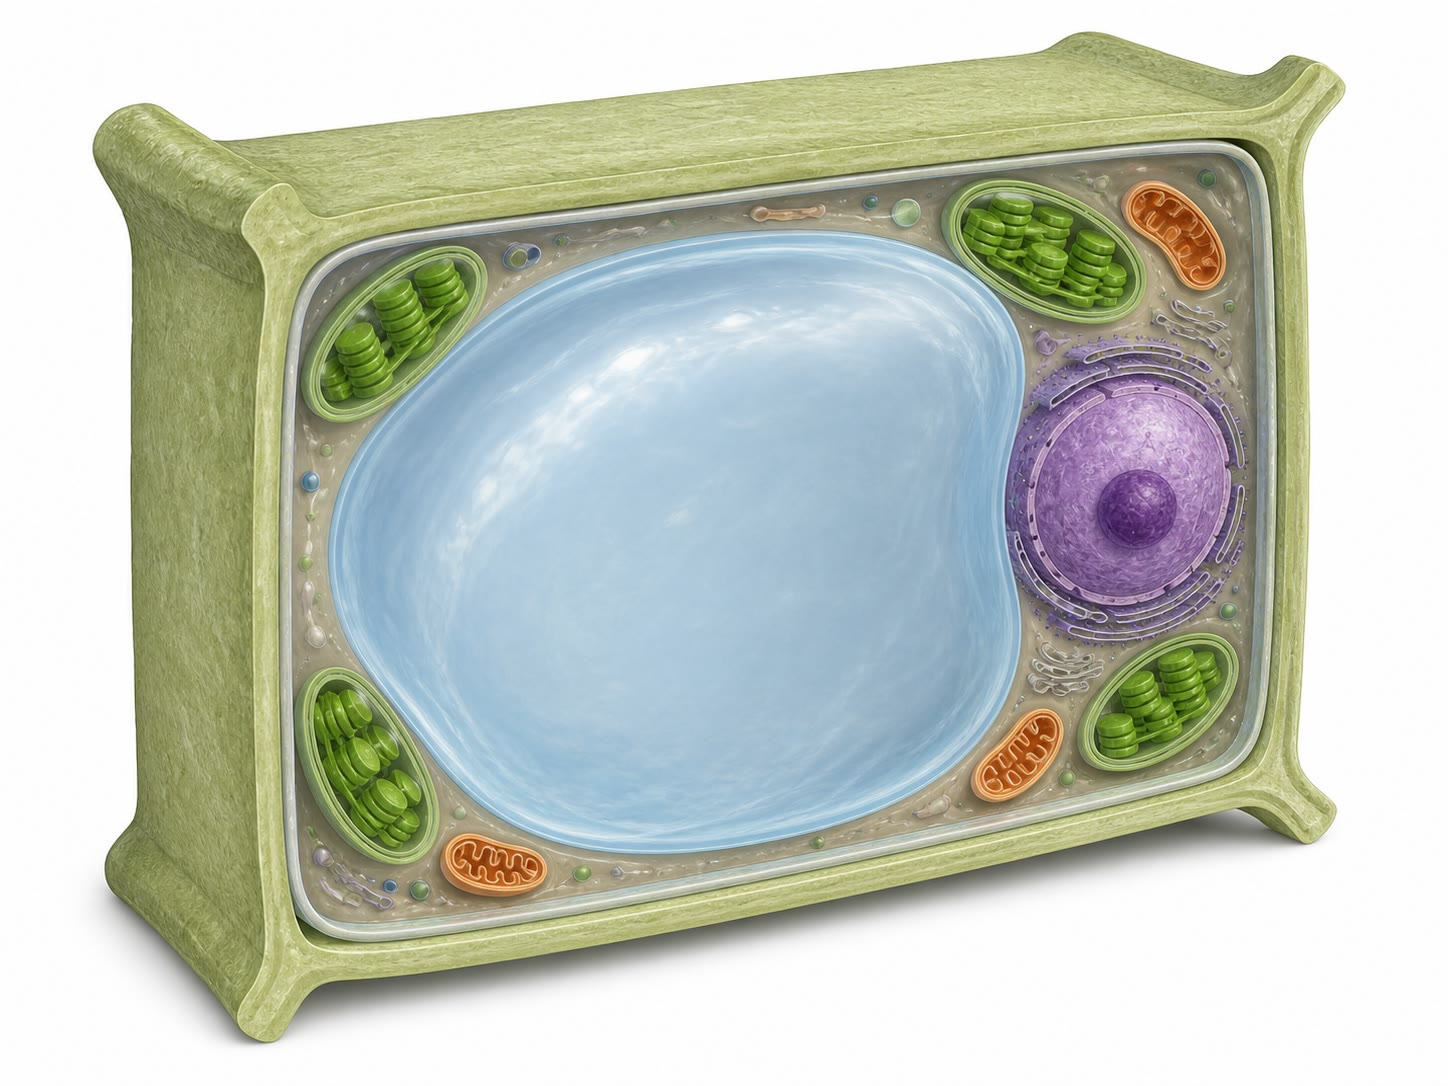
\includegraphics[width=0.52\linewidth]{images/book2/ai/fig-plant-cell-cutaway-v2.jpg}};
  \begin{scope}[x={(img.south east)}, y={(img.north west)},
      every node/.style={font=\small}]
    \draw[omDef, thick] (0.50,0.50) -- (0.50,1.08) node[above] {中央液泡};
    \draw[omDef, thick] (0.10,0.50) -- (-0.03,0.56) node[left] {细胞壁};
    \draw[omDef, thick] (0.25,0.73) -- (-0.03,0.84) node[left] {叶绿体};
    \draw[omDef, thick] (0.35,0.17) -- (-0.03,0.12) node[left] {线粒体};
    \draw[omDef, thick] (0.76,0.47) -- (1.03,0.60) node[right] {细胞核};
    \draw[omDef, thick] (0.60,0.13) -- (1.03,0.16) node[right] {薄层细胞质};
  \end{scope}
\end{tikzpicture}

{\small 植物\omterm{def:b1:cell-unit-of-life:cell}{细胞}：\omterm{def:b1:cell-unit-of-life:cell}{质膜}之外为\omterm{def:b1:eukaryotic-cell:plantcell}{细胞壁}，\omterm{def:b1:eukaryotic-cell:plantcell}{液泡}
占据\omterm{def:b1:cell-unit-of-life:cell}{细胞}的大部分体积，\omterm{def:b1:eukaryotic-cell:plastid}{叶绿体}与\omterm{def:b1:eukaryotic-cell:mitochondrion}{线粒体}位于其间的薄层
\omterm{def:b1:cell-unit-of-life:cell}{细胞质}中。}
\end{omfigure}

\begin{proposition}[植物细胞与动物细胞的比较]\label{prop:b1:eukaryotic-cell:compare}
两者都具有\omterm{def:b1:eukaryotic-cell:nucleus}{细胞核}、\omterm{def:b1:eukaryotic-cell:endomembrane}{内质网}、\omterm{def:b1:eukaryotic-cell:endomembrane}{高尔基体}、\omterm{def:b1:eukaryotic-cell:mitochondrion}{线粒体}、\omterm{def:b1:eukaryotic-cell:peroxisome}{过氧化物酶体}、核糖体
和\omterm{def:b1:eukaryotic-cell:cytoskeleton}{细胞骨架}。植物\omterm{def:b1:cell-unit-of-life:cell}{细胞}具有纤维素\omterm{def:b1:eukaryotic-cell:plantcell}{细胞壁}、大\omterm{def:b1:eukaryotic-cell:plantcell}{液泡}、
\omterm{def:b1:eukaryotic-cell:plastid}{质体}和\omterm{def:b1:eukaryotic-cell:plantcell}{胞间连丝}，没有中心粒和\omterm{def:b1:eukaryotic-cell:endomembrane}{溶酶体}
（\omterm{def:b1:eukaryotic-cell:plantcell}{液泡}承担消化功能）；它不能爬行或吞噬，分裂时
通过在中部构建新的\omterm{def:b1:eukaryotic-cell:plantcell}{细胞壁}完成。动物\omterm{def:b1:cell-unit-of-life:cell}{细胞}没有\omterm{def:b1:eukaryotic-cell:plantcell}{细胞壁}
（因此能够改变形状、爬行并进行吞噬作用），具有\omterm{def:b1:eukaryotic-cell:endomembrane}{溶酶体}、
含中心粒的\omterm{def:b1:eukaryotic-cell:cytoskeleton}{中心体}，并经由连接（而非\omterm{def:b1:eukaryotic-cell:plantcell}{胞间连丝}）相互通讯；
它通过缢缩一分为二进行分裂。
\end{proposition}

\begin{example}[膨压]\label{ex:b1:eukaryotic-cell:turgor}
一个叶\omterm{def:b1:cell-unit-of-life:cell}{细胞}，\omterm{def:b1:eukaryotic-cell:plantcell}{液泡}中溶质为 \qty{0.3}{mol/L}，持续吸水，
直至\omterm{def:b1:eukaryotic-cell:plantcell}{细胞壁}以约 \qty{0.7}{MPa} 的压强反推，
相当于七个大气压；此时\omterm{def:b1:cell-unit-of-life:cell}{细胞}饱满，叶片挺立。失水后，
\omterm{def:b1:eukaryotic-cell:plantcell}{液泡}体积减小，压强降为零，叶片
萎蔫——\omterm{def:b1:eukaryotic-cell:plantcell}{细胞壁}未变，压强已消失
（见\cref{ch:b1:membranes-transport}）。同一溶液中的动物\omterm{def:b1:cell-unit-of-life:cell}{细胞}
因无\omterm{def:b1:eukaryotic-cell:plantcell}{细胞壁}，只会直接胀破。
\end{example}

\section{练习}

\begin{exercise}[$\star$]\label{exo:b1:eukaryotic-cell:1}
列出动物\omterm{def:b1:cell-unit-of-life:cell}{细胞}中的具膜\omterm{def:b1:eukaryotic-cell:organelle}{细胞器}，
并用几句话说明各自的主要功能。
\end{exercise}

\begin{exercise}[$\star$]\label{exo:b1:eukaryotic-cell:2}
追踪一种消化酶从合成到排出\omterm{def:b1:flowering-plant-organization:tissues}{导管}的路径，
指出途经的每个区室，并说明蛋白质如何在它们之间转运。
\end{exercise}

\begin{exercise}[$\star$]\label{exo:b1:eukaryotic-cell:3}
根据膜预算图，\omterm{def:b1:eukaryotic-cell:mitochondrion}{线粒体}膜（外膜加内膜）
占\omterm{def:b1:cell-unit-of-life:cell}{细胞}膜的比例是多少？为什么内膜
比外膜大得多？
\end{exercise}

\begin{exercise}[$\star$]\label{exo:b1:eukaryotic-cell:4}
写出植物\omterm{def:b1:cell-unit-of-life:cell}{细胞}具有而动物\omterm{def:b1:cell-unit-of-life:cell}{细胞}没有的三种结构，
以及动物\omterm{def:b1:cell-unit-of-life:cell}{细胞}具有而植物\omterm{def:b1:cell-unit-of-life:cell}{细胞}没有的两种结构。
\end{exercise}

\begin{exercise}[$\star\star$]\label{exo:b1:eukaryotic-cell:5}
根据脉冲追踪图，标记在\omterm{def:b1:eukaryotic-cell:endomembrane}{内质网}、
\omterm{def:b1:eukaryotic-cell:endomembrane}{高尔基体}和分泌颗粒中分别在何时达到峰值？估算从\omterm{def:b1:eukaryotic-cell:endomembrane}{内质网}到颗粒的转运时间，
以及分泌掉一半标记所需的时间。
\end{exercise}

\begin{exercise}[$\star\star$]\label{exo:b1:eukaryotic-cell:6}
用一种使\omterm{def:b1:eukaryotic-cell:cytoskeleton}{微管}解聚的药物处理\omterm{def:b1:cell-unit-of-life:cell}{细胞}。
预测这将如何影响\omterm{def:b1:eukaryotic-cell:endomembrane}{高尔基体}的位置、囊泡运输、
\omterm{def:b1:cell-unit-of-life:cell}{细胞}分裂以及纤毛的摆动。
\end{exercise}

\begin{exercise}[$\star\star$]\label{exo:b1:eukaryotic-cell:7}
列出\omterm{def:b1:eukaryotic-cell:mitochondrion}{线粒体}起源于细菌的四条证据，
并解释为何\omterm{def:b1:eukaryotic-cell:mitochondrion}{线粒体}仍不能脱离
\omterm{def:b1:cell-unit-of-life:cell}{细胞}独立生存。
\end{exercise}

\begin{exercise}[$\star\star$]\label{exo:b1:eukaryotic-cell:8}
\omterm{def:b1:eukaryotic-cell:endomembrane}{内质网}的腔在拓扑学上“位于\omterm{def:b1:cell-unit-of-life:cell}{细胞}外”。请
通过追踪一种糖链朝向\omterm{def:b1:eukaryotic-cell:endomembrane}{内质网}腔的膜蛋白，从\omterm{def:b1:eukaryotic-cell:endomembrane}{内质网}
转运至\omterm{def:b1:cell-unit-of-life:cell}{质膜}的过程，解释这一说法：
最终糖链朝向哪一侧？
\end{exercise}

\begin{exercise}[$\star\star$]\label{exo:b1:eukaryotic-cell:9}
一个分泌\omterm{def:b1:cell-unit-of-life:cell}{细胞}每天释放 \qty{2000}{} 个直径为 \qty{1}{\micro m} 的
颗粒，经由面积为 \qty{40}{\micro m^2} 的顶端表面。
计算每天新增的膜量，以及
顶端表面需要被回收利用多少次。这说明了什么？
\end{exercise}

\begin{exercise}[$\star\star\star$]\label{exo:b1:eukaryotic-cell:10}
在含有核糖体、分泌蛋白 mRNA 与
氨基酸的试管中，产物为一条 \qty{320}{} 个残基的肽链；加入\omterm{def:b1:eukaryotic-cell:endomembrane}{内质网}小泡后，
出现一条 \qty{300}{} 个残基的肽链，位于
小泡内，且随后加入的蛋白酶不能将其降解。解释
逐一解释这些观察结果，并说明缺失前二十个
残基的突变体会出现什么情况。
\end{exercise}

\begin{exercise}[$\star\star\star$]\label{exo:b1:eukaryotic-cell:11}
某患者的\omterm{def:b1:cell-unit-of-life:cell}{细胞}缺乏一种可降解脂质的\omterm{def:b1:eukaryotic-cell:endomembrane}{溶酶体}酶，
脂质在肿胀的\omterm{def:b1:eukaryotic-cell:endomembrane}{溶酶体}中积累，\omterm{def:b1:cell-unit-of-life:cell}{细胞}随之死亡。解释
这一\omterm{def:b1:cell-unit-of-life:cell}{细胞}生物学机制，说明为何该疾病在膜更新最快的
\omterm{def:b1:cell-unit-of-life:cell}{细胞}中最为严重，并提出注入血液的酶如何到达
\omterm{def:b1:eukaryotic-cell:endomembrane}{溶酶体}。
\end{exercise}

\begin{exercise}[$\star\star\star$]\label{exo:b1:eukaryotic-cell:12}
“\omterm{def:b1:cell-unit-of-life:prokeuk}{真核细胞}是由若干昔日的细菌组成的联合体，
由膜系统将它们维系在一起。”用一段文字讨论，并权衡
内共生学说能解释什么、不能解释什么（\omterm{def:b1:eukaryotic-cell:nucleus}{细胞核}、\omterm{def:b1:eukaryotic-cell:endomembrane}{内质网}、
\omterm{def:b1:eukaryotic-cell:cytoskeleton}{细胞骨架}）。
\end{exercise}

\section{问题：胰腺的腺泡细胞}

\begin{problem}[{周末问题——一种每天分泌相当于自身质量的
蛋白质的细胞：帕拉德时钟、必须回收的膜、
引导蛋白质去向的信号，最终落在
消化酶的转运时间}]
\label{pb:b1:eukaryotic-cell:1}
一个胰腺腺泡\omterm{def:b1:cell-unit-of-life:cell}{细胞}是边长为 \qty{12}{\micro m} 的立方体，其
顶端面（\qty{144}{\micro m^2}，朝向\omterm{def:b1:flowering-plant-organization:tissues}{导管}）与基底面
朝向血液。质量为 \qty{80}{g} 的人类胰腺约含 $\num{8e10}$
个这样的\omterm{def:b1:cell-unit-of-life:cell}{细胞}，每天分泌 \qty{10}{g} 的酶蛋白。一个
分泌颗粒是直径为 \qty{1}{\micro m} 的球体，其中所含
蛋白质浓度为 \qty{200}{mg/mL}。核糖体每
秒可添加 \qty{5}{} 个氨基酸；典型的酶含 \qty{250}{} 个残基，
残基平均质量为 \qty{110}{g/mol}。

\medskip
\noindent\textbf{第一部分——帕拉德时钟。}
本章的脉冲-追踪图给出了标记物位置
随时间的变化。
\begin{enumerate}
  \item 为何脉冲须短暂，而追踪阶段须含大量
        未标记氨基酸的过量？
  \item 读出标记在\omterm{def:b1:eukaryotic-cell:endomembrane}{内质网}、\omterm{def:b1:eukaryotic-cell:endomembrane}{高尔基体}及颗粒中
        达到峰值的时间。
  \item 估算从\omterm{def:b1:eukaryotic-cell:endomembrane}{内质网}到\omterm{def:b1:eukaryotic-cell:endomembrane}{高尔基体}、从\omterm{def:b1:eukaryotic-cell:endomembrane}{高尔基体}到
        颗粒的转运时间。
  \item \qty{60}{min} 时标记物位于何处？为何其中一部分
        已离开\omterm{def:b1:cell-unit-of-life:cell}{细胞}，而大部分仍在颗粒中？
  \item 第二个实验在 \qty{15}{\celsius} 下进行：标记物
        在\omterm{def:b1:eukaryotic-cell:endomembrane}{内质网}中停留超过一小时。请解释。
\end{enumerate}

\medskip
\noindent\textbf{第二部分——蛋白质的质量。}
\begin{enumerate}[resume]
  \item 计算每个\omterm{def:b1:cell-unit-of-life:cell}{细胞}每天分泌的蛋白质质量，单位为皮克。
  \item 计算一个颗粒的体积，以及其所含的
        蛋白质质量。
  \item 计算每个\omterm{def:b1:cell-unit-of-life:cell}{细胞}每天释放的颗粒数，以及
        每分钟释放的颗粒数。
  \item 计算\omterm{def:b1:cell-unit-of-life:cell}{细胞}的体积，并结合密度
        \qty{1.05}{g/cm^3} 计算其质量。它每天分泌的蛋白质占其自身质量的
        比例是多少？
  \item 计算一个颗粒中酶分子的数目
        （阿伏加德罗常数 $\num{6.0e23}$）。
  \item 计算一个核糖体合成一个酶分子所需的时间。
  \item 要完成每日的产量，需要多少个核糖体持续
        工作？请与该\omterm{def:b1:cell-unit-of-life:cell}{细胞}所含的 $\num{4e6}$ 个核糖体
        比较。
\end{enumerate}

\medskip
\noindent\textbf{第三部分——膜。}
\begin{enumerate}[resume]
  \item 计算一个颗粒的膜面积。
  \item 计算每天经由第 8 题中颗粒的胞吐作用，
        送达顶端面的膜量。
  \item 顶端面的面积每天被补充多少次？
        \omterm{def:b1:cell-unit-of-life:cell}{细胞}必须如何处理这部分膜？通过何种过程？
  \item 颗粒膜来自\omterm{def:b1:eukaryotic-cell:endomembrane}{高尔基体}，而\omterm{def:b1:eukaryotic-cell:endomembrane}{高尔基体}的膜又来自
        \omterm{def:b1:eukaryotic-cell:endomembrane}{内质网}。若该\omterm{def:b1:cell-unit-of-life:cell}{细胞}的\omterm{def:b1:eukaryotic-cell:endomembrane}{内质网}具有 \qty{20000}{\micro m^2}
        的膜，相当于多少天的颗粒膜量？
        这说明\omterm{def:b1:eukaryotic-cell:endomembrane}{内膜系统}内的膜回收利用
        有何意义？
  \item 顶端面带有 \qty{2000}{} 个微绒毛，每个直径为
        \qty{0.1}{\micro m}、长为 \qty{1}{\micro m}。它们
        使面积为 \qty{144}{\micro m^2} 的顶端面扩大了多少倍？
\end{enumerate}

\medskip
\noindent\textbf{第四部分——蛋白质上的“地址”。}
\begin{enumerate}[resume]
  \item 一种酶的 mRNA 在不含膜的试管中翻译，
        得到的肽链比颗粒中发现的酶长 \qty{20}{} 个残基。
        多出的残基位于何处，
        它们又是什么？
  \item 有\omterm{def:b1:eukaryotic-cell:endomembrane}{内质网}小泡存在时，产物长度正确，
        位于小泡内部并且不被蛋白酶降解。请解释。
  \item 用\omterm{def:b1:eukaryotic-cell:organelle}{细胞溶胶}中的酶的 mRNA 进行同样的实验，
        得到的产物位于小泡之外且未受保护。请作出结论。
  \item 某突变删除了这二十个残基。预测酶最终
        位于何处，以及\omterm{def:b1:cell-unit-of-life:cell}{细胞}会发生什么变化。
  \item 另一种酶在\omterm{def:b1:eukaryotic-cell:endomembrane}{溶酶体}中而非颗粒中被发现，
        它带有同类的\omterm{prop:b1:eukaryotic-cell:secretory}{信号序列}。第二次分选决定
        应在途径中的何处作出，
        以及通过何种机制完成？请概述。
  \item 用一种阻断 ATP 合成的药物处理\omterm{def:b1:cell-unit-of-life:cell}{细胞}。
        预测脉冲-追踪实验中的标记物会在何处积累，
        并说明两个原因。
  \item 综合第 3 题与第 8 题：处于\omterm{def:b1:organism-environment:homeostasis}{稳态}时，任一时刻有多少颗粒
        正处于\omterm{def:b1:eukaryotic-cell:endomembrane}{内质网}与颗粒之间的“运输途中”？
  \item 总结结果：从合成到颗粒的转运时间，
        分泌所需的时间，每分钟释放的颗粒数，
        以及\omterm{def:b1:cell-unit-of-life:cell}{细胞}每天分泌的蛋白质占自身质量的
        比例。
\end{enumerate}
\end{problem}
